% supplementary.tex — Supplementary material for the bilingual corpus article.
% Compiles on its own: pdflatex supplementary.tex
% Elsevier publishes supplementary files exactly as received, so this file must be final.
\documentclass[11pt]{article}
\usepackage[utf8]{inputenc}
\usepackage[T1]{fontenc}
\usepackage[english]{babel}
\usepackage{lmodern}
\usepackage[margin=2.5cm]{geometry}
\usepackage{booktabs}
\usepackage{tabularx}
\usepackage{graphicx}
\usepackage{amsmath}
\usepackage{xurl}
\usepackage[colorlinks=true,linkcolor=blue,urlcolor=blue]{hyperref}

\renewcommand{\thetable}{S\arabic{table}}
\renewcommand{\thefigure}{S\arabic{figure}}
\renewcommand{\thesection}{S\arabic{section}}
\makeatletter\setlength{\@fptop}{0pt}\makeatother % float-only pages start at the top

\title{Supplementary material for\\[0.3em]
\large Building a Bilingual English--Spanish Parallel Corpus Using Multi-Model LLM Translation with Consensus Review}
\author{Mario Augusto Ram\'irez-Morales \and Esteban Castillo \and David Camilo Corrales \and Victor Adrian Sosa-Hern\'andez}
\date{}

\begin{document}
\maketitle

This document has two parts. Section~\ref{secS:measures} contains the per-dataset measures that the article summarizes in its text, and Section~\ref{secS:config} gives the configuration of the production run: implementation and hardware, the topic categories used for sampling, the parameters, and the prompts. The corpus, the code, and the notebooks are available at \url{https://github.com/vsosahdz/SpanishDBText}.

\section{Corpus measures}
\label{secS:measures}

All measures were computed separately for English and Spanish and for each dataset (WikiText, FEVER, and Europarl), on the 12,003~entries of the released corpus.

\begin{figure}[h!]
\centering
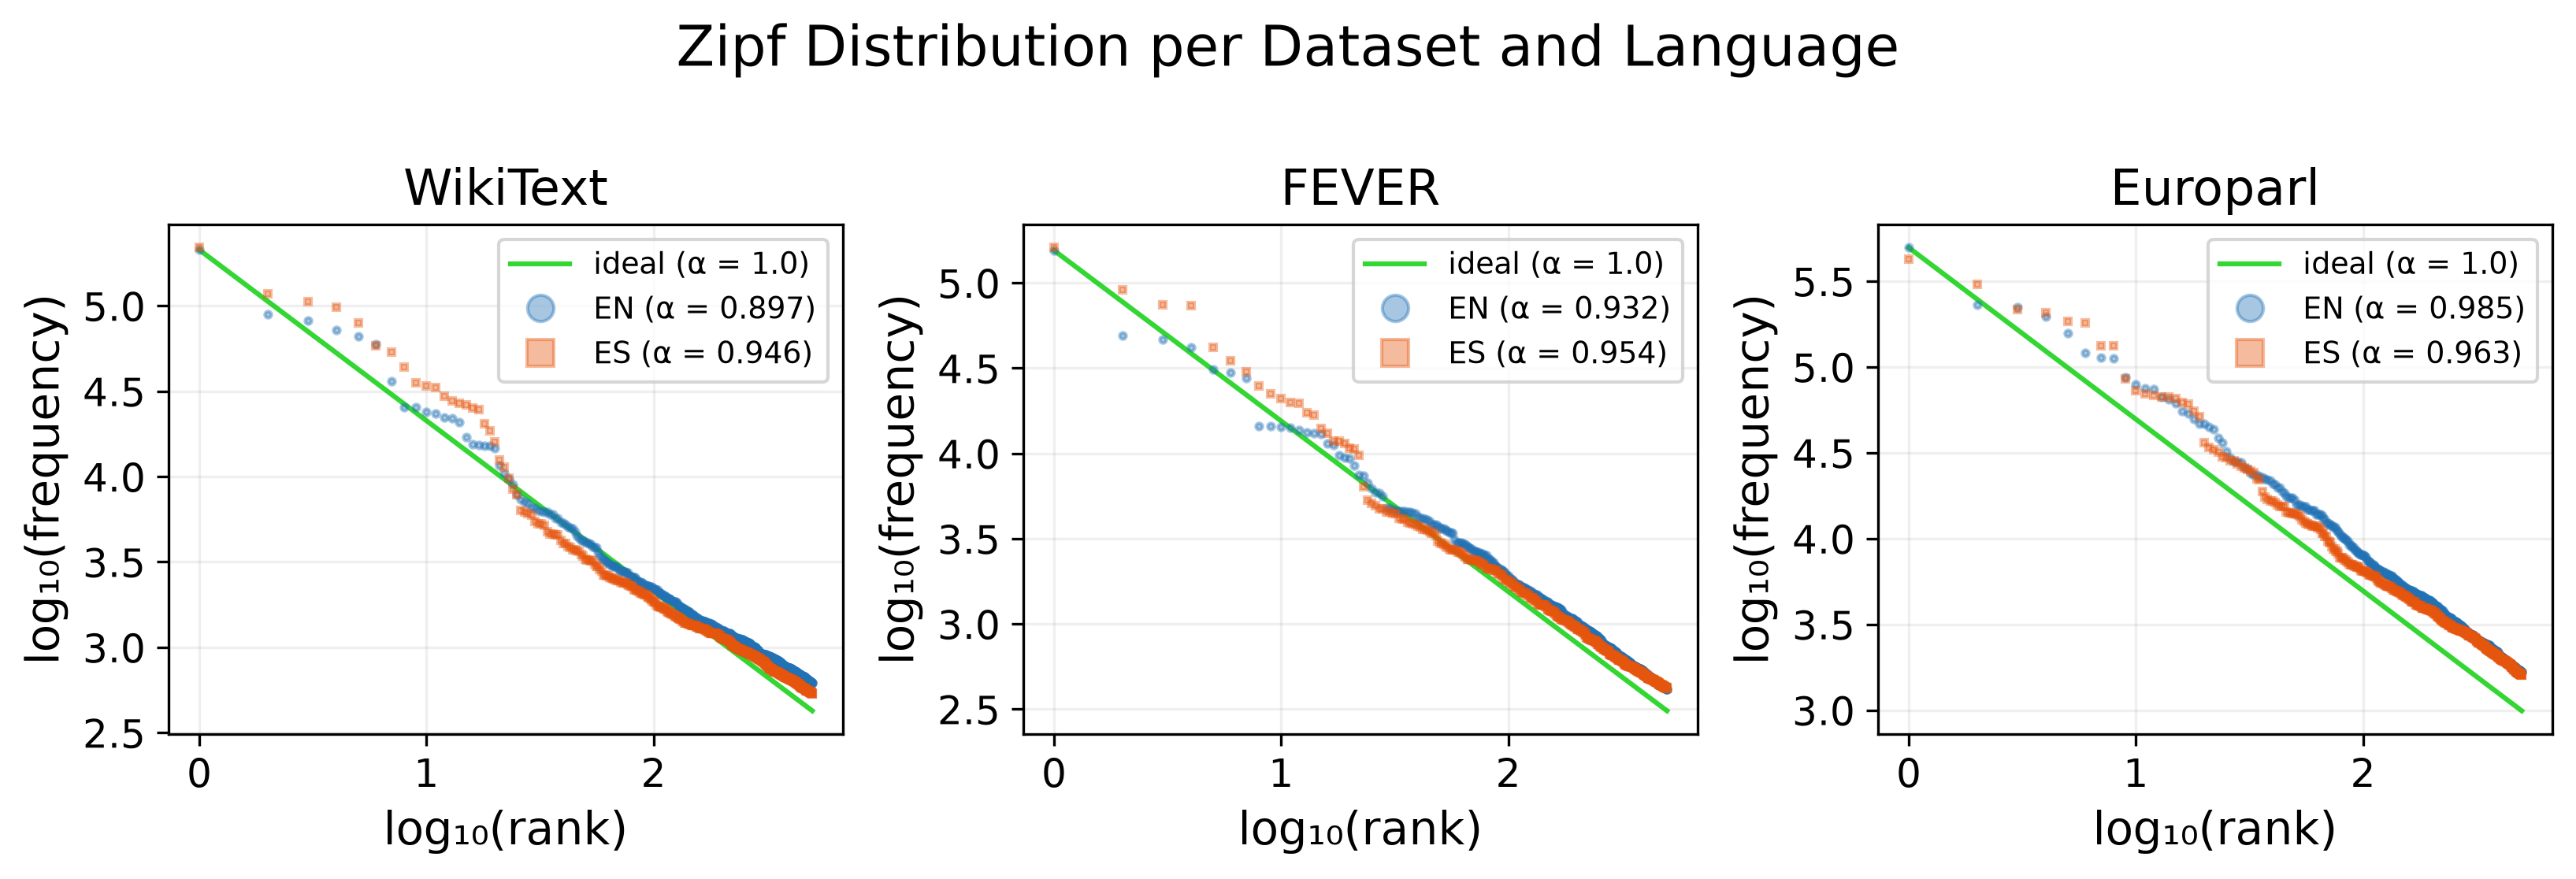
\includegraphics[width=\textwidth]{graphics/zipf_distribution.png}
\caption{Zipf distribution (log-log) per dataset and language. The green line shows the ideal Zipf distribution ($\alpha = 1.0$) as a visual reference. Points above the line are words that appear more often than the ideal predicts (typically function words), and points below it are rare words in the long tail. Both languages follow near-linear trends close to the reference; the fitted exponents (0.89--0.99) are given in the word-frequency table of the article.}
\label{figS:zipf}
\end{figure}

\begin{table}[h!]
\centering
\caption{General corpus statistics per dataset and language: total words, unique words, and words per document. Spanish has 17--57\% more unique words than English in all three datasets.}
\label{tabS:general-stats}
\scriptsize
\begin{tabular*}{\textwidth}{@{\extracolsep{\fill}}@{}llrrrrrr@{}}
\toprule
\textbf{Dataset} & \textbf{Language} & \textbf{Words} & \textbf{Unique} & \multicolumn{4}{c}{\textbf{Words per document}} \\
\cmidrule(lr){5-8}
 & & & & \textbf{Mean} & \textbf{Median} & \textbf{Min} & \textbf{Max} \\
\midrule
WikiText & EN & 2,855,853 & 84,029 & 2,856 & 2,247 & 807 & 8,571 \\
WikiText & ES & 3,038,960 & 104,670 & 3,039 & 2,409 & 872 & 9,438 \\
\midrule
FEVER    & EN & 1,753,843 & 54,057 & 175 & 140 & 76 & 3,554 \\
FEVER    & ES & 1,941,480 & 63,253 & 194 & 156 & 71 & 3,701 \\
\midrule
Europarl & EN & 6,950,546 & 36,790 & 6,916 & 5,886 & 217 & 25,619 \\
Europarl & ES & 6,954,048 & 57,701 & 6,920 & 5,898 & 199 & 26,145 \\
\bottomrule
\end{tabular*}
\end{table}

\begin{table}[h!]
\centering
\caption{Lexical diversity per dataset and language, computed at corpus level. TTR is the type-token ratio, which depends on text length; MATTR (window of 100 words) and MTLD do not. MTLD/doc mean is MTLD averaged over documents.}
\label{tabS:lexical-stats}
\scriptsize
\begin{tabular*}{\textwidth}{@{\extracolsep{\fill}}llrrrr}
\toprule
\textbf{Dataset} & \textbf{Language} & \textbf{TTR} & \textbf{MATTR (w=100)} & \textbf{MTLD} & \textbf{MTLD/doc mean} \\
\midrule
WikiText & EN & 0.029 & 0.708 & 84.63 & 84.69 \\
WikiText & ES & 0.034 & 0.695 & 77.27 & 77.83 \\
\midrule
FEVER & EN & 0.031 & 0.690 & 72.86 & 68.44 \\
FEVER & ES & 0.033 & 0.670 & 63.24 & 61.19 \\
\midrule
Europarl & EN & 0.005 & 0.715 & 89.74 & 89.29 \\
Europarl & ES & 0.008 & 0.717 & 91.47 & 91.54 \\
\bottomrule
\end{tabular*}
\end{table}

\begin{table}[h!]
\centering
\caption{Sentence length per dataset and language, in words. The maximum values are artifacts of the regular-expression sentence splitter on text without standard punctuation, not real sentences.}
\label{tabS:syntactic-stats}
\scriptsize
\begin{tabular*}{\textwidth}{@{\extracolsep{\fill}}llrrrr}
\toprule
& & \multicolumn{4}{c}{\textbf{Sentence length (words)}} \\
\cmidrule(lr){3-6}
\textbf{Dataset} & \textbf{Language} & \textbf{Mean} & \textbf{Median} & \textbf{Standard deviation} & \textbf{Maximum} \\
\midrule
WikiText & EN & 22.0 & 21 & 11.9 & 403 \\
WikiText & ES & 23.8 & 22 & 12.9 & 501 \\
\midrule
FEVER & EN & 21.4 & 20 & 12.8 & 469 \\
FEVER & ES & 24.4 & 22 & 14.4 & 658 \\
\midrule
Europarl & EN & 25.0 & 22 & 15.2 & 1,584 \\
Europarl & ES & 24.9 & 22 & 15.2 & 1,616 \\
\bottomrule
\end{tabular*}
\end{table}

\begin{table}[h!]
\centering
\caption{Quality indicators per dataset and language: character expansion ratio and its standard deviation, exact duplicates within each dataset, and the shares of stopwords and special characters.}
\label{tabS:quality-stats}
\scriptsize
\begin{tabular*}{\textwidth}{@{\extracolsep{\fill}}llrrrrr}
\toprule
\textbf{Dataset} & \textbf{Language} & \textbf{Expansion} & \textbf{Exp.\ std} & \textbf{Duplicates} & \textbf{Stopwords \%} & \textbf{Special \%} \\
\midrule
WikiText & EN & N/A & N/A & 0 & 36.67 & 3.08 \\
         & ES & 1.044 & 0.036 & 0 & 38.71 & 2.47 \\
\midrule
FEVER    & EN & N/A & N/A & 11 & 33.16 & 3.24 \\
         & ES & 1.091 & 0.066 & 0 & 38.89 & 2.44 \\
\midrule
Europarl & EN & N/A & N/A & 0 & 43.16 & 3.23 \\
         & ES & 1.051 & 0.021 & 0 & 40.68 & 3.05 \\
\bottomrule
\end{tabular*}
\par\smallskip\scriptsize Expansion ratio = character length of Spanish / English (shown on the ES row). Duplicates are exact-match counts within each dataset.
\end{table}

\begin{table}[h!]
\centering
\caption{Vocabulary growth as datasets are processed sequentially, per language. Bold marks the Europarl row, which adds the most words of the three datasets but the fewest new ones, and where English and Spanish diverge most. The 100\% values for WikiText are definitional, since it is processed first.}
\label{tabS:growth-curve}
\scriptsize
\begin{tabular*}{\textwidth}{@{\extracolsep{\fill}}llrrrr}
\toprule
\textbf{Dataset} & \textbf{Language} & \textbf{Words Added} & \textbf{Unique After} & \textbf{New Unique} & \textbf{New (\%)} \\
\midrule
WikiText   & EN & 2,855,853 & 84,029  & 84,029 & 100.0 \\
           & ES & 3,038,960 & 104,670 & 104,670 & 100.0 \\
\midrule
+ FEVER    & EN & 1,753,843 & 107,163 & 23,134 & 21.6 \\
           & ES & 1,941,480 & 129,623 & 24,953 & 19.3 \\
\midrule
+ Europarl & EN & \textbf{6,950,546} & 117,297 & \textbf{10,134} & \textbf{8.6} \\
           & ES & \textbf{6,954,048} & 150,745 & \textbf{21,122} & \textbf{14.0} \\
\bottomrule
\end{tabular*}
\end{table}

\clearpage
\section{Pipeline configuration}
\label{secS:config}

This section gives the configuration of the production run that the article summarizes in its Implementation and Pipeline Configuration sections. The code and the full text of every prompt are in the repository.

\subsection{Implementation and hardware}

The pipeline is written in Python~3.11+ and uses no NLP or translation libraries. API calls are made with httpx, and the translation models run in parallel with Python's ThreadPoolExecutor. Model assignments, provider credentials, and generation parameters (temperature, context window, and output limit) are read from a \texttt{.env} file; the other thresholds and the retry counts are constants in the pipeline code. Subset selection and corpus analysis were done in Jupyter notebooks with pandas and NumPy, and all outputs are stored as JSON files.

We ran the whole production from one laptop: an 8-core AMD Ryzen~9 8945HS with 32~GB of RAM and an NVIDIA RTX~4060 Laptop GPU with 8~GB of VRAM, under Windows~11. The same machine served Qwen~3.5~9B with Ollama inside a Docker container. The other five model roles were reached through Azure OpenAI and Azure AI Foundry.

\subsection{Topic categories for stratified sampling}

WikiText and FEVER, both taken from Wikipedia, share 14 categories: music, military history, sports, film and television, geography and places, science, transport, biography, politics and government, nature and weather, technology, history, religion and philosophy, and \emph{other}. Europarl uses 15 categories adapted to parliamentary business: economy and finance, institutional affairs, foreign affairs, trade and market, environment and energy, human rights, transport and infrastructure, development aid, agriculture and food, justice and security, social affairs and employment, health and consumers, digital technology, defence, and \emph{other}.

Each entry goes to the category whose keyword list has the most matches in the entry, or to \emph{other} when no keyword matches. The text matched against the keyword lists differs by source. For WikiText and FEVER, it is the title plus the first 2,000 characters of the body; for Europarl, it is the debate title alone, because the title of a session already states its subject.

\subsection{Parameters}

Table~\ref{tabS:parameters} lists the parameters of the run. We used a temperature of 0.2 for all models, so that translations are mostly stable but can vary slightly. A value of 0 would remove all variation, and higher values would add randomness to a task that requires fidelity to the source. The context window (32,768 tokens) and the maximum output (8,192 tokens for translation and review, 1,024 for evaluation and metadata) are the limits supported by the models used. The article explains the chunking values in its Pipeline Configuration section.

We set the API timeout at 600 seconds (10 minutes) for the local Qwen model, which is much slower than the cloud models on long chunks. The override margin of 10 points means that the programmatic truncation check replaces the completeness score of the evaluator only when the two differ widely, which avoids corrections for small differences. The 40\% weight of completeness in the overall score reflects the priority given to missing content: truncation is a more serious problem than minor issues of fluency or clarity.

\begin{table}[h!]
\centering
\caption{Key pipeline parameters.}
\label{tabS:parameters}
\footnotesize
\begin{tabular}{llr}
\toprule
\textbf{Parameter} & \textbf{Scope} & \textbf{Value} \\
\midrule
Temperature & All models & 0.2 \\
Context window & All models & 32,768 tokens \\
Max output & Translation, Review & 8,192 tokens \\
Max output & Evaluation, Metadata & 1,024 tokens \\
Chunking threshold & Stage~2 & 6,000 est. tokens \\
Max chunk size & Stage~2 & 12,000 characters \\
API timeout & All calls & 600 seconds \\
Max retries & All calls & 3 \\
Language retries & Stage~3 & 2 \\
Truncation ratio threshold & Stage~5 & 0.92 \\
Truncation override margin & Stage~5 & 10 points \\
Completeness weight & Stage~5 & 40\% \\
\bottomrule
\end{tabular}
\end{table}

\subsection{Prompts}

Every LLM call has a \emph{system prompt}, which defines the model's role and fixed rules, and a \emph{user prompt}, which provides the text of each entry and any extra context. Table~\ref{tabS:prompts} lists all the prompts of the pipeline.

\begin{table}[h!]
\centering
\caption{Prompt inventory: structural components and corpus-specific variants.}
\label{tabS:prompts}
\renewcommand{\arraystretch}{1.15}
\scriptsize
\begin{tabularx}{\textwidth}{@{}p{2.6cm}XXp{1.5cm}p{1.8cm}@{}}
\toprule
\textbf{Prompt} & \textbf{System layer} & \textbf{User layer} & \textbf{Output} & \textbf{Variants} \\
\midrule
Translation system (St.~3)      & Role + 10 fidelity/style rules            & Source text + direction                     & Plain text       & 3 (WT, F, EP) \\
Language retry user (St.~3)     & (same as translation)                     & Error notice + source text                  & Plain text       & 1 per direction \\
\midrule
Critique system + user (St.~4a) & Role + JSON schema requirement            & Orig.\ + candidates                         & JSON             & 1 (shared) \\
Merge system + user (St.~4b)    & Role + fidelity/completeness rules        & Orig.\ + candidates + critique              & Plain text       & 1 (shared) \\
\midrule
Evaluation system + user (St.~5) & Role + scoring guide + completeness rules & Orig.\ + translation + char lengths + ratio & JSON            & 1 (shared) \\
\midrule
Metadata system + user (St.~6)  & Role + format instruction                 & 4-field template + article text             & Structured lines & 2 (EN, ES) \\
\bottomrule
\end{tabularx}
\renewcommand{\arraystretch}{1}
\end{table}

\paragraph{Translation.} The translation system prompt gives the model a professional role (``You are a professional translator specialized in editorial and technical translation'') and sets ten rules. They cover semantic fidelity (no invention, omission, or addition), natural output, a neutral professional Spanish register not tied to any national variety, preservation of technical terms and proper nouns, respect for the original tone and paragraph structure, and a ban on markdown formatting that is not in the original.

There are three variants of this system prompt, one per corpus, which keep the same role and core rules and adapt them to the structure of each corpus. The WikiText variant adds rules to remove the \texttt{=} signs of section headers and the \texttt{<unk>} tokens of the dataset. The FEVER variant adds a sports terminology rule: use the established Spanish term when one exists (e.g., \emph{tiro libre} for \emph{free throw}, \emph{ponchar} for \emph{strikeout}), and keep the English term only when none exists. The Europarl variant replaces the WikiText cleaning rules with an instruction to keep all XML structural tags (\texttt{<CHAPTER>}, \texttt{<SPEAKER>}, \texttt{<P>}) intact and untranslated.

The user prompt is a short wrapper that provides the text and states the translation direction. When language validation finds output in the wrong language, the retry user prompt reports the error (e.g., ``Your previous response was in English. You MUST translate the following text to Spanish'') and repeats the original text.

The system prompts for translation, review, and evaluation are written in Spanish, to orient the model toward the target language. Only the metadata stage has one system prompt per language, one in Spanish and one in English, because it extracts metadata from both the source and the translation.

\paragraph{Review.} The critique system prompt asks the reviewer to analyze each candidate, list its strengths and weaknesses, and give it a score from 0 to 100. It must return a JSON object that also names the base candidate and the improvements to apply. The critique user prompt supplies the original text and the candidates in clearly marked sections. The merge system prompt then asks the reviewer to write the final translation from the original text, the candidates, and the critique. Its rules repeat the fidelity and completeness rules of the translation prompt, and its output is plain text. The critique runs once per entry, and its choice of base candidate applies to the whole entry. The merge runs once per segment for entries that were split, at the same boundaries as the chunks.

\paragraph{Evaluation.} The evaluation system prompt asks for strict scoring (a perfect score must be extremely rare) and contains the scoring guide of the article. It also sets completeness rules: if the translation is much shorter than the original (character ratio below 0.85), it is probably truncated, and a truncated translation cannot receive more than 70 for completeness. The user prompt gives the character counts of both texts and their ratio, and adds a warning when the ratio is below 0.85. The output is a JSON object with the four dimension scores, a list of errors, and an overall score.

\paragraph{Metadata.} The metadata system prompt combines a minimal role with a strict format requirement. It has two variants, one in Spanish for the translation and one in English for the source, so that the model works in the language of the text it analyzes. The user prompt is a fixed template with one line per field (title, keywords, topic, and summary), format limits for each field, and the text in a separate, clearly marked block. The pipeline parses the answer with regular expressions. Each corpus has its own topic list (Table~\ref{tabS:metadata-taxonomy}), and all three lists end with an open option (``or other appropriate'').

\begin{table}[h!]
\centering
\caption{Topic categories offered to the metadata model in Stage~6, per corpus. Each list ends with an open-ended ``or other appropriate'' option.}
\label{tabS:metadata-taxonomy}
\footnotesize
\begin{tabularx}{\textwidth}{@{}lX@{}}
\toprule
\textbf{Corpus} & \textbf{Categories} \\
\midrule
WikiText-103 & video game, novel, biography, science, history, technology, politics, medicine, sports, entertainment \\
FEVER & sports, music, film, history, politics, science, geography, biography, technology, religion, military, transport \\
Europarl & politics, legislation, economy, environment, human rights, agriculture, defense, trade, health, technology \\
\bottomrule
\end{tabularx}
\end{table}

\end{document}
